\section{Simulation}
Le but est de générer une matrice d'adjacence A sous les mêmes hypothèses que \eqref{eq:1} en faisant varier les différents paramètres, à savoir: $n$, $p_{in}$, $p_{out}$ \\

\begin{figure}[H]
\centering
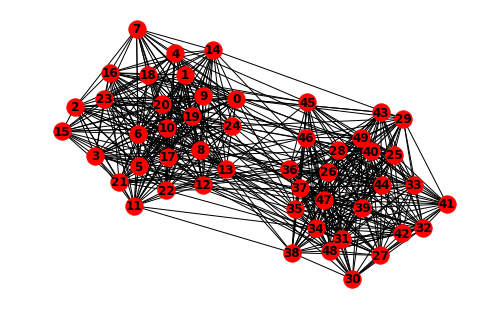
\includegraphics[scale=0.6]{static/graph_n50_pin08_pout01.png}
\caption{Graphe généré à partir des paramètres: $n=50$, $p_{in}=0.8$, $p_{out}=0.1$}
\end{figure}

L'élément discriminant du test spectral étant la variable $ \Delta p= p_{in} - p_{out}$, nous allons tester 3 valeurs représentatives des différents types de résultats:
\begin{itemize}
	\item[1-] $\Delta p \in [-1,\: -p_{lim}] \implies$ le graphe comporte de structure de communauté ``disassortative'';
	\item[2-] $\Delta p \in [-p_{lim},\: p_{lim}] \implies$ la méthode spectrale ne peut rien conclure sur la stucture de communauté du graphe;
	\item[2-] $\Delta p \in [p_{lim},\: 1] \implies$ le graphe comporte une structure de communauté ``assortative''.\\
\end{itemize}

Par la suite nous allons tester pour les valeurs $\Delta p= 0.5, 0.08, -0.5$ .
De plus nous ferons une première batterie de test avec $n=100$ et une autre avec $n=1000$.
La terminologie utilisée dans les figures ci-dessous est:
\begin{itemize}
	\item[- \underline{$n,\: p_{in},\: p_{out},\: p_{lim},\: z_1,\: z_2$}:] sont identiques aux notations utilisées jusqu'à présent ;
	\item[- \underline{$z_1\: theoric, \:z_2\: theoric$}:] sont les plus grandes valeurs propres $z_1$ et $z_2$ calculées via les équations \eqref{z_1} et \eqref{z_2} ;    
	\item[- \underline{$p_{in}\: estimated, \:p_{out}\: estimated$}:] sont les probabilités du SBM calculées a posteriori grâce aux valeurs propres $z_1$ et $z_2$.\\
\end{itemize}
Les $p_{in}\: estimated, \:p_{out}\: estimated$ sont calculés via un calcul d'optimisation.\\
\begin{figure}[p]
	\begin{subfigure}{.5\textwidth}
		\centering
		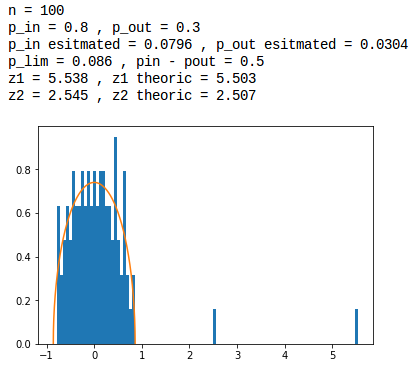
\includegraphics[scale=0.58]{static/spectral_n100_pin08_pout03.png}
		\caption{$n=100$, $\Delta p=0.5$}
		\label{n100delta05}
	\end{subfigure}
	\begin{subfigure}{.5\textwidth}
		\centering
		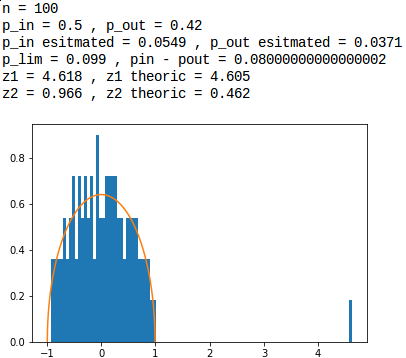
\includegraphics[scale=0.58]{static/spectral_n100_pin05_pout042.png}
		\caption{$n=100$, $\Delta p=0.08$}
		\label{n100delta008}
	\end{subfigure}
	\begin{subfigure}{.5\textwidth}
		\centering
		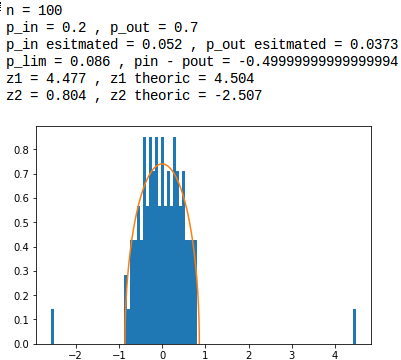
\includegraphics[scale=0.58]{static/spectral_n100_pin02_pout07.png}
		\caption{$n=100$, $\Delta p=-0.5$}
		\label{n100delta-05}
	\end{subfigure}
	\begin{subfigure}{.5\textwidth}
		\centering
		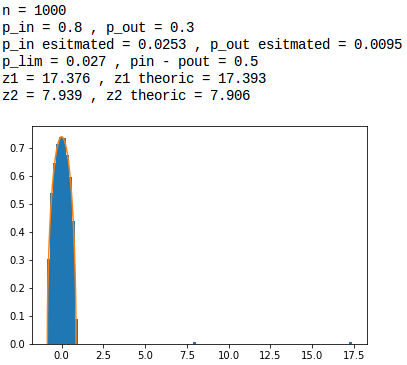
\includegraphics[scale=0.58]{static/spectral_n1000_pin08_pout03.png}
		\caption{$n=1000$, $\Delta p=0.5$}
		\label{n1000delta05}
	\end{subfigure}
	\begin{subfigure}{.5\textwidth}
		\centering
		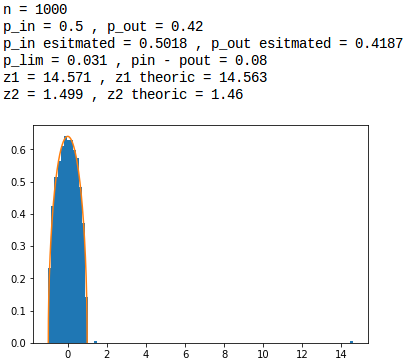
\includegraphics[scale=0.58]{static/spectral_n1000_pin05_pout042.png}
		\caption{$n=1000$, $\Delta p=0.08$}
		\label{n1000delta008}
	\end{subfigure}
	\begin{subfigure}{.5\textwidth}
		\centering
		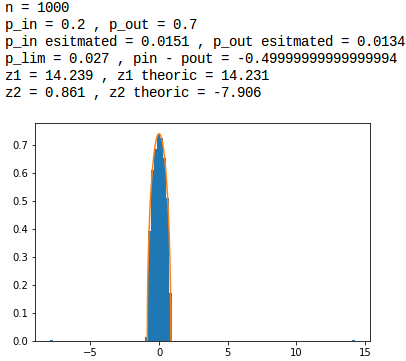
\includegraphics[scale=0.58]{static/spectral_n1000_pin02_pout07.png}
		\caption{$n=1000$, $\Delta p=-0.5$}
		\label{n1000delta-05}
	\end{subfigure}
\end{figure}

La première observation que l'on peut faire est que les valeurs propres de nos matrices d'adjacence sont bien distribuées selon la loi du demi-cercle de Wigner.
De plus, en fonction de $\Delta p$ la mesure spectrale est perturbé (ou pas) par une ou deux valeurs propres qui sortent du support de la distribution initiale.\\

Dans les cas avec $\Delta p = 0.5$ (\autoref{n100delta05}, \autoref{n1000delta05}), on voit très clairement deux valeurs propres qui se détachent du support de la distribution de Wigner.
Les valeurs $z_1$, $z_2$ correspondent bien aux valeurs théoriques avec un taux d'erreur de l'ordre de $10^{-2}$.
Par conséquent lorsque l'on obtient une valeur propre négative, le modèle spectral nous permet de conclure qu'il y a une structure de communauté ``assortative'' dans le graphe.\\

Dans les cas avec $\Delta p = -0.5$ (\autoref{n100delta008}, \autoref{n1000delta008}), selon l'\autoref{z_2}, on ne s'attend à ce qu'une des valeurs propres théorique soit négative.
On observe une valeur propre négative en dehors du support de la loi de Wigner et une autre au dessus du support.
Ces valeurs observées correspondent on valeurs théoriques avec une erreur de l'ordre de $10^{-2}$.
Par conséquent lorsque l'on obtient une valeur propre négative, le modèle spectral nous permet de conclure qu'il y a une structure de communauté ``disassortative'' dans le graphe.\\

Enfin, les cas avec $\Delta p = 0.08$ (\autoref{n100delta-05}, \autoref{n1000delta-05}). 
On se trouve dans le cas limite décrit dans \autoref{subsec:1.3}, dans lequel le modèle ne peut pas interpréter les résultats du modèle spectral.
On peut observer sur la \autoref{n100delta-05} qu'il n'y a qu'une seule valeur propre qui est en dehors du support.
Par conséquent il n'y a qu'une seule valeur propre extrémale (ici $z_1$) qui correspond à sa valeur théorique, de fait nous ne pouvons conclure sur la structure de communauté du graphe.
Cependant, avec le même $\Delta p$ mais avec plus de nœud ($n = 1000$) le modèle spectral parvient à détecter la structure de communauté et à retrouver les valeurs $z_1$ et $z_2$.  
Ceci confirme la remarque du \autoref{rq:ngrand} selon laquelle, plus il y a d’information (i.e nœuds) dans le graphe plus la valeur de $p_{lim}$ tend vers $0$.\\

Si on compare les valeurs théoriques de l'article initial \cite{raj_rao} avec les valeurs des simulations, on voit très clairement une différence.\\
Par exemple, pour $p_{in} = 0.8$, $p_{out}=0.3$, et $n=100$ les valeurs propres calculées avec les équations \nameref{tab:bilan} sont $z_1 = 22.785$ et $z_2 = 18.815$.
Les valeurs propres empiriques sont $z_1 = 5.538$ et $z_2 = 2.545$.\\
Ou encore, pour $p_{in} = 0.2$, $p_{out}=0.7$, et $n=1000$ les valeurs propres calculées avec les équations \nameref{tab:bilan} sont $z_1 = -56.732$ et $z_2 = 31.833$.
Les valeurs propres empiriques sont $z_1 = 14.299$ et $z_2 = -7.934$.